% this file is called up by thesis.tex
% content in this file will be fed into the main document

\chapter{Compression model}
\label{ch:exprlang}


% ----------------------- paths to graphics ------------------------

\graphicspath{{4_expression_language/images/}}

% ----------------------- contents from here ------------------------
% 

\textit{Whitebox compression} is a compression model for columnar database systems. Its purpose is to represent data more compactly through elementary operator expressions. These operators---chained together into expression trees---form the expression language used for data representation. This chapter describes the \textit{whitebox compression} model, its expression language and operators, the structure of expression trees and their evaluation.

\section{Expression language}
\label{sec:exprlang:exprlang}

The \textit{whitebox} compression model represents logical columns as composite functions of physical columns. We refer to these functions as \textit{operators}. With respect to databases, logical columns are columns as seen by the database user, containing the data in its original format. Physical columns contain the physical representation of the data as it is stored on disk, in a different format.

Formally, we define an operator as a function \(o\) that takes as input zero or more columns and optional metadata information and outputs a column: 
\begin{equation}
\label{eq:exprlang:exprlang:operator}
    o \colon [C \times C \times ...] \times [M] \to C
\end{equation}

The domain of \(o\) is composed of columns and metadata and the codomain is columns. A column is defined by its datatype \(d\) and the values that it contains \(V\). The metadata is structured information of any type.

We defined our expression language based on a set of elementary column representation types, each having an associated operator. They are listed in Table~\ref{tab:exprlang:exprlang_1}.

\begin{table}[h]
\centering
\makebox[\textwidth][c]{
\begin{tabular}{l|rll}
\multicolumn{1}{c|}{Representation} & \multicolumn{3}{c}{Operator}                                                                                          \\ \hline
Concatenation of 2 or more columns  & \(concat \colon\) & \multicolumn{1}{l|}{\(C \times C \times [...] \to C\)} & \(c = concat(c_a, c_b, [...])\)          \\ \hline
Formatting of another column        & \(format \colon\) & \multicolumn{1}{l|}{\(C \times M \to C\)}              & \(c = format(c_a, m_{\mathit{format}})\) \\ \hline
Direct mapping of another column    & \(map \colon\)    & \multicolumn{1}{l|}{\(C \times M \to C\)}              & \(c = map(c_a, m_{map})\)                \\ \hline
Constant representation             & \(const \colon\)  & \multicolumn{1}{l|}{\(M \to C\)}                       & \(c = const(m_{const})\)                
\end{tabular}
}
\caption{Elementary column representation types}
\label{tab:exprlang:exprlang_1}
\end{table}

The concatenation of two string columns \(c_a\) and \(c_b\) is the concatenation of each pair of values \(v_a\) and \(v_b\). E.g. \(\verb|"123abc"| = \mathit{concat}(\verb|"123"|, \verb|"abc"|)\), where \(v_a = \verb|"123"|\) and \(v_b = \verb|"abc"|\). The representation of a string column \(c_a\) as a formatted non-string column \(c_b\) consists of the individual values \(v_b\) formatted as strings based on the format string metadata \(m_{\mathit{format}}\). This can be seen as datatype change. E.g. 
\(\verb|"-12000"| = \mathit{format}(\verb|-12000|, \verb|"%d"|)\), where \(v_b = \verb|-12000|\)
and 
\(m_{\mathit{format}} = \verb|"%d"|\)
. The direct mapping representation of a column \(c_a\) as a column \(c_b\) through the mapping \(m_{map}\) is a key-value lookup in a dictionary-like data structure. E.g. \(\verb|"valueoncolumnA"| = dict[\verb|"valueoncolumnB"|]\), where \verb|valueoncolumnB| is the key and \verb|"valueoncolumnA"| is the value in the dictionary \verb|dict|. The constant representation of a column indicates that all its values are equal to the constant value \(m_{\mathit{const}}\). The \(\mathit{const}\) operator just returns \(m_{\mathit{const}}\).

These operators and transformations can be composed, resulting in operator expressions. For example, the logical columns \(A\) and \(B\) in Table~\ref{tab:exprlang:exprlang_2}, can be represented as composite functions of the physical columns in Table~\ref{tab:exprlang:exprlang_2}, through the following expressions:
\begin{equation}
\label{eq:exprlang:exprlang:example}
\begin{array}{ll}
    A &= \mathit{concat}(\mathit{map}(P, {dict_{AP}}), \mathit{const}(\verb|"_"|), \mathit{format}(Q, \verb|"%d"|))\\
    B &= \mathit{map}(P, {dict_{BP}})
\end{array}
\end{equation}

\begin{table}[h]
\centering
\begin{minipage}{.75\linewidth}
\centering
\begin{tabular}{@{}ll@{}}
\toprule
\multicolumn{1}{c}{A} & \multicolumn{1}{c}{B}                    \\ \midrule
\verb|"GSA_8350"|     & \verb|"GENERAL SERVICES ADMINISTRATION"| \\
\verb|"GSA_8351"|     & \verb|"GENERAL SERVICES ADMINISTRATION"| \\
\verb|"HHS_2072"|     & \verb|"HEALTH AND HUMAN SERVICES"|       \\
\verb|"TREAS_4791"|   & \verb|"TREASURY"|                        \\
\verb|"TREAS_4792"|   & \verb|"TREASURY"|                        \\
\verb|"HHS_2073"|     & \verb|"HEALTH AND HUMAN SERVICES"|       \\
\verb|"GSA_8352"|     & \verb|"GENERAL SERVICES ADMINISTRATION"| \\ \bottomrule
\end{tabular}
\caption*{Logical columns}
\end{minipage}%
\begin{minipage}{.25\linewidth}
\centering
\begin{tabular}{@{}cc@{}}
\toprule
P        & Q           \\ \midrule
\verb|0| & \verb|8350| \\
\verb|0| & \verb|8351| \\
\verb|1| & \verb|2072| \\
\verb|2| & \verb|4791| \\
\verb|2| & \verb|4792| \\
\verb|1| & \verb|2073| \\
\verb|0| & \verb|8352| \\ \bottomrule
\end{tabular}
\caption*{Physical columns}
\end{minipage}
\caption{Whitebox representation example: data}
\label{tab:exprlang:exprlang_2}
\end{table}

\begin{table}[h]
\centering
\begin{minipage}{.25\linewidth}
\centering
\begin{tabular}{@{}ll@{}}
\toprule
key      & value          \\ \midrule
\verb|0| & \verb|"GSA"|   \\
\verb|1| & \verb|"HHS"|   \\
\verb|2| & \verb|"TREAS"| \\ \bottomrule
\end{tabular}
\caption*{\(dict_{AP}\)}
\end{minipage}%
\begin{minipage}{.6\linewidth}
\centering
\begin{tabular}{@{}ll@{}}
\toprule
key      & value                                    \\ \midrule
\verb|0| & \verb|"GENERAL SERVICES ADMINISTRATION"| \\
\verb|1| & \verb|"HEALTH AND HUMAN SERVICES"|       \\
\verb|2| & \verb|"TREASURY"|                        \\ \bottomrule
\end{tabular}
\caption*{\(dict_{BP}\)}
\end{minipage}
\caption{Whitebox representation example: metadata}
\label{tab:exprlang:exprlang_3}
\end{table}

We observe that column \(A\) has the following structure: a dictionary compressible prefix and a numeric suffix, separated by a the '\verb|_|' character. If we store these logical parts separated into 3 columns \(C_{\mathit{prefix}}\), \(C_{\mathit{delim}}\), \(C_{\mathit{suffix}}\), we can represent column \(A\) as their concatenation. Since \(C_{\mathit{prefix}}\) has repeated values, we can represent it more compactly as the mapping of column \(P\)---containing dictionary keys---and the dictionary \(dict_{AP}\)---presented in Table~\ref{tab:exprlang:exprlang_3}. We can represent \(C_{\mathit{delim}}\) through the \textit{const} operator since all its values are equal to '\verb|_|'. \(C_{\mathit{suffix}}\) contains numbers stored in strings. We can store these values more compactly as numbers, by changing the column datatype. Therefore, we represent \(C_{\mathit(suffix)}\) based on the numeric column \(Q\), through the \(format\) operator, with the format string \verb|"%d"|. We move our attention to column \(B\) and observe that it is correlated with column \(C_{\mathit{prefix}}\)---and implicitly also to column \(P\). We can therefore represent \(B\) as the mapping of column \(P\) and the dictionary \(dict_{BP}\)---presented in Table~\ref{tab:exprlang:exprlang_3}. In the end, we store only the physical columns \(P\) and \(Q\) and the metadata: \(dict_{AP}\), \(dict_{BP}\) and the constant string \verb|"_"|. The original values on the logical columns \(A\) and \(B\) can be reconstructed by evaluating the expressions in Equation~\ref{eq:exprlang:exprlang:example}.

So far, we described 4 column representation types and their associated operators: \(concat\), \(format\), \(map\) and \(const\). The \textit{whitebox compression} model does not limit itself to these representation types. It is a generic model and supports any type of column operators (e.g. mathematical operators like addition or multiplication). A practical example is the \textit{whitebox} version of the Frame of Reference compression method: \(const(\mathit{reference}) + C_{\mathit{diff}}\), where \(+\) is the numeric addition/sum operator, \(\mathit{reference}\) is the reference value and \(C_{\mathit{diff}}\) is the physical column containing the differences between the original values and \(\mathit{reference}\).

The purpose of \textit{whitebox compression} is to represent data more compactly through elementary operator expressions similar to the ones presented above. However, there are a multitude of different possible representations of the same logical columns, each one giving a different result. We will describe the optimization problem of finding the best representation for a set of columns in \ref{subsec:learningprocess:optimizationproblem}~\nameref{subsec:learningprocess:optimizationproblem}.

These operator expressions create more compact representations of logical columns, exploiting the underlying compression opportunities in the data. We showed how we can remove redundancy from data by representing columns as functions of other columns through the \(map\) operator and how we can store numeric values in more suitable datatypes through the \(format\) operator. We are able to decompose string columns into subcolumns with values from different distributions, thus enabling independent representations. Finally, the key factor of the \textit{whitebox} model is that it allows recursive representation of columns, ultimately leading to improved compression ratios.

\section{Expression tree}
\label{sec:exprlang:exprtree}

The operators presented so far are useful for describing the data representation and for transforming the physical data into its original logical format. We call this process \textit{decompression}. In practice, we need to transform the logical data into its physical format first---\textit{compression}. The compression process requires a different expression, one that represents the physical columns as functions of the logical columns, through the inverse operators of the ones presented until now. Table~\ref{tab:exprlang:exprlang_4} presents the compression operators types.

\begin{table}[h]
\centering
\small
\makebox[\textwidth][c]{
\begin{tabular}{@{}lrll@{}}
\toprule
\multicolumn{1}{c}{Transformation}      & \multicolumn{3}{c}{Operator}                                                                      \\ \midrule
Split a column into multiple columns    & \(split \colon\)   & \(C \to C \times C \times [...]\) & \(split(c) = c_a, c_b, [...]\)           \\
Change datatype of a column             & \(cast \colon\)    & \(C \times M \to C\)              & \(cast(c, m_{\mathit{datatype}}) = c_a\) \\
Direct mapping of another column        & \(map \colon\)     & \(C \times M \to C\)              & \(map(c, m_{map}) = c_a\)                \\
Consume a column (constant/correlation) & \(consume \colon\) & \(C \times M \to \emptyset\)      & \(consume(c, m) = \emptyset\)            \\ \bottomrule
\end{tabular}
}
\caption{Compression operator types}
\label{tab:exprlang:exprlang_4}
\end{table}

All these operator types and their practical implementations will be discussed in detail in \ref{sec:pd}~\nameref{sec:pd}. For now, we are interested in their definition. We notice how the formal definition of the compression operator is different from the one of the compression operators:
\begin{equation}
\label{eq:exprlang:exprtree:operator:comp}
    o \colon C \times [M] \to [C \times C \times ...]
\end{equation}

The compression operators take as input a single column and compression metadata information and output 0 or more columns. Because of the multiple column output, representing physical columns as composite functions of logical columns is not straightforward. Therefore, we introduce the concept of \textit{expression trees}, as an alternative representation instead of the nested operator expressions.

\textit{Expression trees} are tree-like structures with 2 types of nodes: \textit{column nodes} and \textit{operator nodes}. We also use the term \textit{expression node} to refer to the \textit{operator nodes}---they are interchangeable. An \textit{expression tree} is composed of alternating levels of \textit{column} and \textit{operator} nodes. Root nodes are always \textit{column nodes}. Leaf nodes can be either \textit{column nodes} or \textit{operator nodes}---in the case of operators that do not output any column. An \textit{operator node} in an \textit{expression tree} is the equivalent of and operator in an operator expression: it has input columns---connected through incoming edges---and output columns---connected through outgoing edges. \textit{Expression trees} are used in the compression and decompression processes as more practical alternatives to the operator expressions. To better understand the similarities between the two, we created the equivalent \textit{expression tree} of the operator expressions for columns \(A\) and \(B\) in Equation~\ref{eq:exprlang:exprlang:example}. Recall the expressions: \(A = \mathit{concat}(\mathit{map}(P, {dict_{AP}}), \mathit{const}(\verb|"_"|), \mathit{format}(Q, \verb|"%d"|))\) and \(B = \mathit{map}(P, {dict_{BP}})\). The equivalent \textit{expression tree} is presented in Figure~\ref{fig:exprlang:exprtree:tree_1}.

\begin{figure}[h]
  \centering
  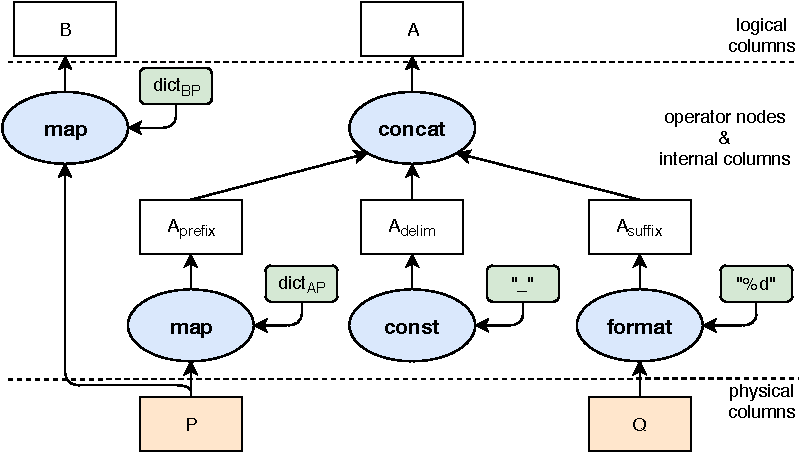
\includegraphics[width={0.9\linewidth}]{expression_language-tree_1_1.pdf}
  \caption{Expression tree representation}
  \label{fig:exprlang:exprtree:tree_1}
\end{figure}

The first thing to notice is that the \textit{expression tree} is not actually a tree, but an acyclic directed graph with 2 root nodes. However, we chose to stick to the term \textit{expression tree} instead of graph, since it is more intuitive. In this case the graph is connected, but in other cases it can have multiple connected components. For example, imagine that in our example we had an additional logical column \(C\) that is represented as a function of a physical column \(S\), without any connection with the columns or operators used to represent columns \(A\) and \(B\). Then, our graph will have 2 connected components. 

Besides the graph-like structure, the \textit{expression tree} is an equivalent representation of the operator expressions. We notice the similarities between the operator nodes and the operators in the nested expressions and the alternating levels of columns and operators. A noticeable difference is the additional columns \(A_{\mathit{prefix}}\), \(A_{\mathit{delim}}\) and \(A_{\mathit{suffix}}\). These are non-materialized internal columns that make the recursive representation possible. In terms of representation type, this is a \textit{decompression tree}, since the root nodes are the physical columns \(P\) and \(Q\) and the expression nodes are decompression operators. The \textit{compression tree} will have the same structure, only that the root nodes will be the logical columns \(A\) and \(B\) and the expression nodes will be compression operators. The metadata will also differ.

There is the case that different subsets of the values on a column come from different distributions and cannot be represented through the same expression. E.g. a string column where odd rows contain the same constant value and even rows are numbers. These situations are common in real data, as we have seen in the Public BI benchmark, where there are not many columns for which a single representation perfectly fits all the values. One option to accommodate these cases is to allow a single column to be represented through multiple operators. In terms of \textit{decompression trees}, the column will have multiple incoming edges each one from a different operator. These multi-representation structures need to be explicitly handled in the \textit{expression tree} evaluation process (described in \ref{sec:exprlang:compdecomp}~\nameref{sec:exprlang:compdecomp}). The second option of handling these cases is through recursive representation of \textit{exception columns}, which is discussed in \ref{sec:exprlang:exceptions}~\nameref{sec:exprlang:exceptions}.

\section{Exception handling}
\label{sec:exprlang:exceptions}

While analyzing the Public BI benchmark in search for patterns and \textit{whitebox compression} opportunities we noticed that columns where all values perfectly fit the same pattern/representation are not very common. Instead there is a smaller or larger subset of values that do not fit the dominant pattern of the column. Lets take for example the data in Table~\ref{tab:exprlang:exprlang_2}. Image that a few values on column \(A\) did not have the \verb|prefix-delim-suffix| structure and instead they were just arbitrary strings. Then, the representation in Figure~\ref{fig:exprlang:exprtree:tree_1} could not be applied on the entire column. We call these values that do not match the representation: \textit{exceptions}. In the \textit{whitebox compression} model \textit{exceptions} are stored on separate \textit{exception columns}. These are nullable columns that contain \verb|null| on positions where the value was not an exception and the original values otherwise. Conversely, the non-exception columns are also nullable and contain null on the positions of exceptions.

We defined 2 ways of handling \textit{exceptions}: 1) through the multi-representation approach mentioned in \ref{sec:exprlang:exprlang}~\nameref{sec:exprlang:exprlang}; 2) through recursive representation of \textit{exception columns}. The first option implies having an operator expression for each subset of values that requires a separate representation. The second option implies choosing a single representation, storing \textit{exceptions} on a separate \textit{exception column} and then recursively applying the same process on the \textit{exceptions}. The two options are equivalent from the physical data perspective. Only the shape of the tree differs: flat and wide trees in the first case and deeper trees in the second case. An additional difference between the two options is the number of \textit{exception columns}: the first option requires at most one \textit{exception column} for every logical column (to store values that do not fit any pattern), while the second option implies having a separate \textit{exception column} for each operator node in the expression tree. The two approaches are illustrated in Figure~\ref{fig:exprlang:exceptions}.

\begin{figure}[h]
\centering
\makebox[\textwidth][c]{
\begin{subfigure}[t]{0.49\linewidth}
  \centering
  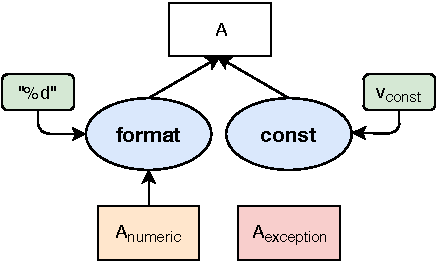
\includegraphics[width={1.0\linewidth}]{4_expression_language/images/expression_language-exceptions_1_option_1.pdf}
  \caption{Multi-representation}
  \label{fig:exprlang:exceptions:option1}
\end{subfigure}
\hspace{3em}
\begin{subfigure}[t]{0.31\linewidth}
  \centering
  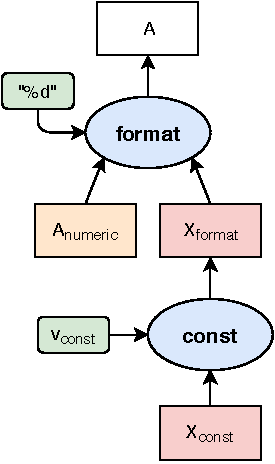
\includegraphics[width={1.0\linewidth}]{4_expression_language/images/expression_language-exceptions_1_option_2.pdf}
  \caption{Recursive exception representation}
  \label{fig:exprlang:exceptions:option2}
\end{subfigure}
}
\caption{Representation options \& exception handling}
\label{fig:exprlang:exceptions}
\end{figure}

Figure~\ref{fig:exprlang:exceptions} shows the 2 equivalent representations of a string column \(A\), which has 2 major subsets of values: one containing numeric values and the other one a constant value. The figure on the left shows the multi-representation approach: the 2 operators are on the same level of the tree and the exceptions---i.e. the values that do not fit any of the 2 representations---are stored separately in the \(A_{\mathit{exception}}\) column. \(A_{\mathit{numeric}}\) and \(A_{\mathit{exception}}\) are both physical columns. The figure on the right shows the recursive exception representation: the subset of numeric values are represented through the \(format\) operator and the rest are rejected to the \textit{exception column} \(X_{\mathit{format}}\). \(X_{\mathit{format}}\) now contains the subset of constant values, and is represented through the \(const\) operator. The remaining values which are not constant are stored in the \(X_{\mathit{const}}\) \textit{exception column}. The physical columns in this case are \(A_{\mathit{numeric}}\) and \(X_{\mathit{const}}\), while \(A_{\mathit{format}}\) is just an intermediate non-materialized \textit{exception column}. The 2 representations are equivalent in terms of the physical data structure: the numeric values are stored in \(A_{\mathit{numeric}}\) and the exceptions---values that are neither numeric nor constant---are stored in the \(A_{\mathit{exception}}\) respectively \(X_{\mathit{const}}\) column.

In our implementation we used a combination of the 2 approaches: select the dominant patterns in the data and represent each column through multi-representation expressions and then store the rest of the values---which do not fit the representations---in \textit{exception columns}. If there are more opportunities left in the exceptions, recursive representation of the \textit{exception columns} is implicitly performed by the compression learning algorithm, since they are treated as normal columns.

\iffalse
- exceptions can also contain patterns; can be recursively compressed with other methods
- 2 options: 1) a single exception column per logical column (unable to recursively compress exceptions, thus we need multi-representation structures in the tree); 2) an exception column for each operator: allowing recursive compression of exceptions and implicitly used multiple representations for the same column
\fi

\section{Compression and decompression}
\label{sec:exprlang:compdecomp}

The evaluation of a \textit{compression tree} on a set of logical columns---i.e. \textit{compression}---means applying the operators on the logical values in order to generate the physical values that will be stored in the physical columns. Conversely, the evaluation of a \textit{decompression tree} on a set of physical columns---i.e. \textit{decompression}---is the process of applying the operators on the physical values to obtain the original data. The 2 process are similar and we will further discuss only \textit{decompression}.

Given a table with multiple logical columns, its expression tree (graph) will have 1 or more connected components. Each component can be evaluated independently from the other components. The decompression process starts from the root nodes and evaluates the operators on the path to the target logical/physical column, in topological order. In the case of \textit{decompression}, exceptions are handled by checking for \verb|null| values on the \textit{exception column}. If the value at a given position on the \textit{exception column} is not \verb|null| then it was an exception, otherwise the operator needs to be evaluated. A special case is when a logical data value is \verb|null| and also an exception. For this case we use a bitmap indicating which values were \verb|null| in the first place. In the case of \textit{compression}, the operators are responsible for deciding which values are exceptions and which are not: if an operator throws an exception then the value is stored on the \textit{exception column}. The \textit{compression} and \textit{decompression} processes are similar for the multi-representation structures defined in the previous sections. For \textit{compression}, the decision upon which representation fits a given value is determined by the (first) operator that does not raise an exception. If all operators raise an exception then the value is stored on the \textit{exception column}. For \textit{decompression}, the physical columns that do not contain \verb|null| values indicate the representation of each value. This process is similar to the SQL \verb|COALESCE| function \cite{sqlcoalesce}, which returns the first non-null value in a list of expressions.

The process of evaluating \textit{expression trees} in topological order is suitable for vectorized execution \cite{kersten2018everything} and SIMD instructions since the elementary operators can be evaluated in the same order for blocks of data, generating intermediate results which fit in the cache. Alternatively, JIT compilation \cite{kersten2018everything} can be used to generate compiled code for each component of the expression tree during compression time, which is then executed for each query. However, the scope of this thesis does not cover fast evaluation of expression trees. We leave this topic for future work.


% \section{Representation example}
% \label{sec:exprlang:repexamples}

% TODO-1: give example from PBIB with compression ratio and compressed execution opportunity (the one in the presentation)

% \iffalse
% - expression tree examples & compression ratio calculation + compressed execution potential; also mention thesis focus (not compressed execution)
% \fi


% ---------------------------------------------------------------------------
% ----------------------- end of thesis sub-document ------------------------
% ---------------------------------------------------------------------------

\iffalse
where:
\begin{itemize}
    \item[] \(n\) = total number of expression nodes
    \item[] \(c_{in}\) = number of input columns
    \item[] \(p\) = number of pattern detectors
    \item[] \(n_{p}\) = number of expression nodes returned by a pattern detector
    \item[] \(b\) = branching factor of the compression tree
    \item[] \(h\) = height of the compression tree
    \item[] \(c_{out}\) = number of output columns of an expression node
\end{itemize}
\fi